\chapter{CEES: Classification of Energy-efficient Settings}

This chapter describes CEES (\textbf{C}lassification of \textbf{E}nergy-\textbf{e}fficient \textbf{S}ettings), focusing on the High Performance Computing (HPC) domain.
Energy and power consumption will be first-class constraints in future exascale systems \cite{exaosr-power}.
For example, these systems are predicted to have strict operating budgets of approximately 20 MW \cite{Exascale20MW}.
Additionally, exascale operating systems are required to actively ``decrease the cost per scientific insight'' \cite{DOEML}.  
Minimizing application energy, even if runtime is increased, can: (1) greatly reduce the cost (in Joules) of scientific insight, and (2) increase application throughput in over-provisioned, power-constrained systems---such as future exascale computers \cite{PatkiRMAP,Sarood2013}---by allowing more applications to execute on a cluster simultaneously.

We propose to dynamically monitor application and system behavior at runtime and use machine learning classification to predict the most energy-efficient resource settings as the application executes.
% In this context, energy efficiency is the ratio of work completed to energy consumed---effectively, the runtime cost of performing a fixed-size computation.
The proposed approach has two distinct benefits.
First, it can be applied to new applications without modifying either the classifier or application, as it does not require application-level instrumentation or hooks.
Second, classification's low overhead makes it suitable for running in-situ on compute nodes.


\section{Motivation}
\label{sec:classifiers-motivation}

We first describe how maximizing energy efficiency is distinct from maximizing performance or minimizing power consumption.
As such, finding the most energy-efficient system setting requires new techniques.
We then discuss the challenges of learning a model for mapping application/system behavior to energy-efficient system settings.


\subsection{Energy Efficiency is a Unique Challenge}

Energy efficiency is the ratio of work completed per unit of energy consumed.
For example, HPC clusters can formulate energy efficiency as the ratio of applications completed per Joule of energy used.
If an application execution represents some unit of scientific insight, then this metric expresses the cost of scientific insights in terms of operational costs (energy consumption).
Thus, maximizing energy efficiency directly reduces the cost of scientific insight by minimizing application energy consumption.

Some recent energy-aware approaches in HPC reduce energy consumption while maintaining application performance \cite{Jitter,Marathe2015,RountreeAdagio}.
As these approaches do not trade application speed, they reduce energy strictly by reducing power.
While it is tempting to use the same approaches to minimize energy by simply removing the constraint on application runtime, failing to account for the impact of lower-power resource settings on execution time can result in worse energy consumption.
Also, while raising processor clockspeed typically reduces application runtime, the requisite increase in power results in increased energy consumption (recall \eqnref{bg-power} in \secref{intro-description}).
In short, maximizing energy efficiency \emph{does not} mean using as little power as possible \emph{or} running as fast as possible---it requires finding the optimal tradeoff between execution time and power consumption.


Typical resource management approaches in HPC clusters primarily attempt to optimize application completion time, only worrying about power consumption to the extent that the total cluster power constraint is not violated, and ignoring energy consumption altogether.
Although there are various techniques for assigning jobs to nodes, minimizing their runtime is usually achieved by running the individual compute nodes as fast as possible, \ie the \emph{race-to-idle} heuristic.
Using \emph{race-to-idle} makes resource scheduling on a node easy, but it is never as energy-efficient as a more intelligent approach that understands how system settings affect performance and power tradeoffs on a per-application basis \cite{kim-cpsna2015}.
\emph{Racing} to finish a job as fast as possible minimizes execution time, but the increase in power dwarfs the time savings, resulting in high energy consumption.

In addition to reducing costs, maximizing energy efficiency will also improve overall system throughput in power-constrained environments.
In over-provisioned clusters, the hardware can draw more total power than the infrastructure can physically deliver to the system if nodes use \emph{race-to-idle} \cite{Sarood2013}.
Effectively, power is now the primary factor limiting cluster size and throughput, not available compute resources.
More aggressively trading performance and power means that optimizing energy efficiency increases total cluster throughput by: (1) allowing more applications to run in parallel due to lower per-application power consumption, while (2) still considering application runtime due to its impact on energy consumption.
Therefore, new resource management approaches are required that focus solely on minimizing energy to reduce the cost of science (in Joules), even if application runtime is increased.


\subsection{Learning Energy Efficiency}
\label{sec:challenges-learning}

Identifying energy-efficient combinations of resource settings is challenging as there is no universal best setting for a system---it depends on the application and its configuration, even varying for different inputs.
Even in a parallel system with homogeneous nodes and perfectly uniform application behavior, optimal settings can vary dramatically due to manufacturing variation \cite{Acun2016}.
Furthermore, many applications progress through different \emph{phases} during execution.
For example, an application may transition between compute and memory-intensive processing, causing the most energy-efficient setting to change during runtime.
It is therefore not optimal to choose a single setting statically when launching the application, necessitating a dynamic approach instead.

We explore learning approaches that adjust system settings to minimize energy.
Specifically, we tune socket allocation, the use of HyperThreads, and processor DVFS.
The learning component picks settings for the combination of these resources such that, at any point during the application execution, the system is operating in its most energy-efficient state.

Our goal is for the learner to find the most energy-efficient setting without requiring any application-level changes.
We therefore use existing hardware performance counters as \emph{features}.
The learner then determines a function that maps some subset of these features into the most energy-efficient system setting.
However, system settings in modern compute nodes have very complicated interactions, so it is essential to use learning mechanisms that can produce accurate mappings despite this complexity.

\begin{figure}[t]
% \vskip -1.0em
\centering
\subfloat[Training data only.]
{\centering 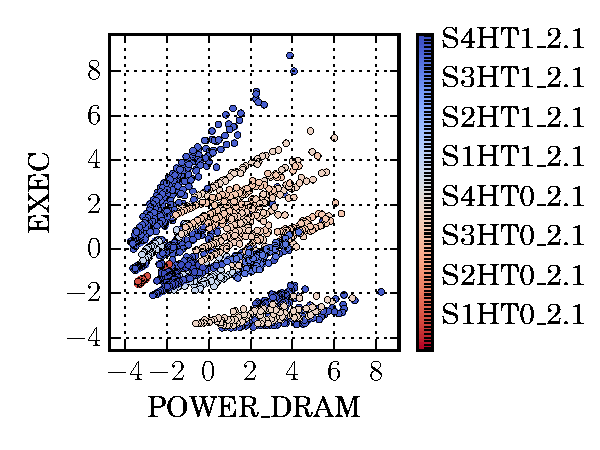
\includegraphics[width=0.3\columnwidth]{figs/classifiers/training_space_noclassifier.pdf}
\label{fig:feat-space-none}
% \vspace{ -1.5em }
}
\hspace*{0.1cm}
% \vskip -1.5em
\subfloat[SVM (Linear kernel), recall=0.456.]
{\centering 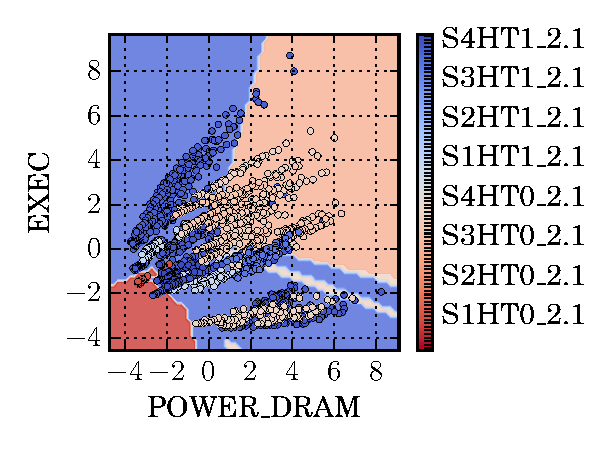
\includegraphics[width=0.3\columnwidth]{figs/classifiers/training_space_svm_kern_lin.pdf}
\label{fig:feat-space-svm-kern-lin}
% \vspace{ -1.5em }
}
\hspace*{0.1cm}
\subfloat[SVM (RBF kernel), recall=0.710.]
{\centering 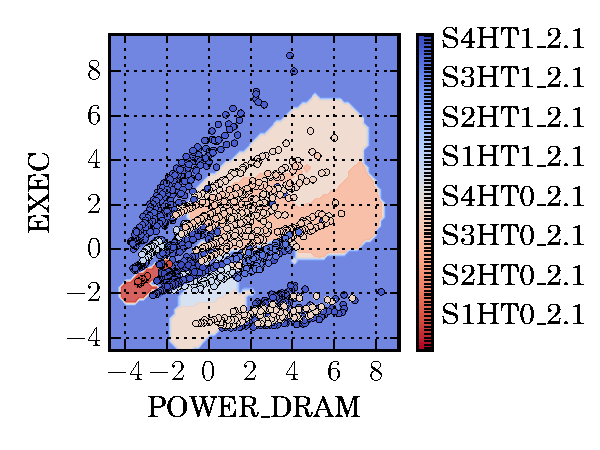
\includegraphics[width=0.3\columnwidth]{figs/classifiers/training_space_svm.pdf}
\label{fig:feat-space-svm}
% \vspace{ -1.5em }
}
\caption{Training data and learned decision boundaries for two SVM classifiers using two primary features.}
\label{fig:feat-space-intro}
% \vskip -1.0em
\end{figure}

We briefly illustrate this complexity using just two features---the performance counters \pc{POWER\_DRAM} (a measure of memory usage) and \pc{EXEC} (a measure of CPU usage).
\figref{feat-space-none} visualizes the behavior of our training data (21 common HPC benchmarks) with respect to normalized performance counter values.
Each data point is the average recorded \pc{POWER\_DRAM} and \pc{EXEC} behavior for a training application running in a single resource configuration on our evaluation system.
There are 88 unique resource configurations, or possible \emph{labels}, accounting for different combinations of the socket count \texttt{S}, whether HyperThreads \texttt{HT} are used, and the DVFS frequency (\eg 2.1\GHz).
% Thus, each application has 88 data points.
All 88 data points belonging to a particular application are assigned \emph{the same label}---the resource configuration with the best average energy efficiency for that application; \ie all 88 data points for an application have the same color.
With this labeling, a good learner will recognize suboptimal behavior and produce the most energy-efficient settings to use instead.
The problem is clearly complex---no intuitive pattern emerges that obviously maps CPU and memory usage into the most energy-efficient system settings.

To successfully map these features into accurate predictions, the learner must be able to handle this complexity, which not all learning mechanisms can.
Consider \figref{feat-space-svm-kern-lin}, which illustrates the accuracy of a Support Vector Machine (SVM) classifier using a linear kernel.
The shaded regions indicate the label (system settings) that the SVM classifier predicts for a range of feature values; the training data is overlaid for comparison.
This linear SVM's \emph{recall}---the fraction of system settings that are accurately predicted when simply replaying the training data---is only 45.6\%, a clear indication that this classifier is not effective.
In contrast, \figref{feat-space-svm} demonstrates a SVM with a radial basis function (RBF) kernel, which achieves 71.0\% recall---better, though perhaps still with room for further improvement.
Note that recall is simpler than cross-validation, since the classifier already saw the same input during supervised training.
If a classifier cannot perform accurate recall, it will likely perform even worse in deployment, when it is exposed to data it has not yet seen.

\section{Classifying System Settings}
\label{sec:classifiers-framework}

We propose to predict energy-efficient settings at runtime, without the overhead of estimating the behavior of all possible system settings before producing a result.
As with many prior works in managing power/energy in HPC systems, we use hardware performance counters to measure application and system behavior.

\begin{figure}[t]
  \begin{centering}
    \tikzset{%
  app/.style    = {draw, thin, rectangle, minimum height = 2em,
    minimum width = 2em, fill=black!25},
  block/.style    = {draw, thick, rectangle, minimum height = 2.5em,
    minimum width = 2.5em},
  blockres/.style    = {draw, thick, rectangle, minimum height = 2.5em,
    minimum width = 2.5em, fill=green!25},
  biblock/.style  = {draw, thick, rectangle, minimum height = 5.5em,
    minimum width = 6em, fill=red!25},
  sum/.style      = {draw, circle, node distance = 2cm}, % Adder
  input/.style    = {coordinate}, % Input
  output/.style   = {coordinate} % Output
}

\begin{tikzpicture}[scale=1.0,transform shape, auto, thick, node distance=1.5cm, >=triangle 45]

\draw
  % Drawing the top blocks
  % node [input, name=goalaccuracy] {} 
  % node [left of=goalaccuracy, node distance=0.35mm]{}
  % node [sum, right of=goalaccuracy] (sumaccuracy) {} % negative feedback
  node [block, align=center] (featureselection) 
    {Feature\\Selection}
  node [block, right of=featureselection, align=center, node distance=3.9cm] (classifier) 
    {Classifier}
  node [blockres, above of=classifier, align=center, node distance=1.8cm] (trainingdata) 
    {Training\\Data}
;
  % Connectng lines
% \draw[->](goalaccuracy) -- node[align=center] {Timing\\Goal}(sumaccuracy);
% \draw[->](sumaccuracy) -- node[align=center] {Timing\\Error}(featureselection);
\draw[->](featureselection) -- node[align=center] {Processed\\Data}(classifier);
\draw[->](trainingdata) -- (classifier);

% Draw software system
\draw
  node [biblock, right of=classifier, node distance=5.2cm, align=center] (system)
    {Compute\\Node\\\\}
;
\draw
  node [app, right of=classifier, node distance=5.2cm, align=center, yshift=-0.5cm] (software)
    {Application}
;

% lines from translators to software
\draw[->](classifier.east) -- node [name=ka,align=center]{System\\Settings} (classifier.east -| system.west);

% Connectng lines
\coordinate (feedbackup) at ([yshift=-0.5cm]featureselection.south);
\draw (system.west |- feedbackup) -| node [near end,align=center] {PCM\\Sample} (feedbackup);
\draw[->](feedbackup) -- node[pos=0.99] {} (featureselection);

\end{tikzpicture}
    \caption{Design for using machine learning classifiers to predict energy-efficient system settings based on performance counter behavior.}
    \label{fig:classifier-runtime}
  \end{centering}
% \vskip -1.0em
\end{figure}

\figref{classifier-runtime} demonstrates our proposed approach.
While an \textbf{application} runs on the \textbf{compute node}, hardware performance counters are polled in the background at regular intervals.
For our experiments, we use the PCM tool to collect performance counter data \cite{PCMGit}.
The \emph{PCM sample} data is scaled, then processed using Principal Component Analysis (PCA) to identify which fields correlate well with energy efficiency.
We also use \textbf{feature selection} to limit the number of hardware counters used by the classifier to reduce runtime overhead (evaluated in \secref{eval-clf-settings}).
Using this \emph{processed data}, the \textbf{classifier} predicts the most energy-efficient \emph{system settings} to use, which are then actuated on the system.
The process then repeats at the next time interval.


\subsection{Training Data}

% \TODO{Figure: Training approach as a pipeline diagram?}

A classifier must be trained before it can be used.
To collect training data, we characterize the behavior of various benchmark applications on the target platform by running them in all possible settings while collecting hardware performance counter results.
In other words, if there are $N$ different allowable settings, each application is executed $N$ times, or once in each setting.
If $M$ applications are used in training, then there are a total of $N \times M$ data points in the training set.
More precisely, each data point is a feature vector, composed of average performance counter values for an execution.

Characterization can be time-consuming, but only needs to be done once for a platform and can be completed in a reasonable period of time by keeping application execution times short.
Choosing applications that are representative of those that will be used on the system improves the likelihood that the classifier can accurately predict settings during runtime.
Additionally, training applications should be chosen that exercise the system hardware components in different patterns to cover a wide range of possible use cases.
% As with most statistical techniques, more data typically leads to better results.

Application energy efficiency (EE) is defined as the amount of work completed per unit of energy (J) used.
Low-level hardware performance counters do not have a metric for quantifying true application progress (work completed), but the instructions retired by the system (INST) is a suitable proxy.
The classifier then quantifies energy efficiency as:
\begin{eqnarray}
EE = \frac{INST}{J}
\label{eqn:ee}
\end{eqnarray}
Each application has a single most energy-efficient setting, so the $N$ executions for the $M$ training set applications are labeled with that setting:
\begin{eqnarray}
% Label = \argmax_{i \in \{1, \ldots, N\}}EE_i
Label[m][n] = \argmax_{i \in N}EE_i \,\,\,\,\,\,\forall m \in M,\,\,\forall n \in N
\label{eqn:label}
\end{eqnarray}
% A label can take any form, \eg a setting index or string name, so long as the actuator knows how to interpret it.
Ideally, total instruction count would be fixed for an application execution, then this proxy for computing energy efficiency would align with true application execution energy efficiency.
However, instruction count typically increases with the application execution time, \eg due to background processes like PCM or kernel tasks.
As such, it is important to note that labeling the most energy-efficient configuration using \eqnref{label} is different than using the minimum-energy execution from the training set.
There are two reasons for using instruction count in computing energy efficiency.
First, energy efficiency can be quantified at any point during an execution, making it a useful metric for runtime behavior analysis.
Second and more importantly, \eqnref{ee} is a function of events happening \emph{at the time}.
Total energy requires knowing all events that \emph{will} happen during the application execution, introducing the possibility that the classifiers might be learning something about application input rather than the way hardware events correspond to energy consumption.
Accounting for instructions helps to avoid this pitfall.


\subsection{Performance Counters}
\label{sec:perf-counters}

Performance counter metrics are available at different levels of granularity---system, socket, and core.
For simplicity, we limit ourselves to system-wide data.
\tblref{pcm} lists the performance counters that we process for our experiments \cite{PCMFields}.

\begin{table}[t]
\caption{Overview of system-level performance counters.}
\label{tbl:pcm}
\small
\centering
\begin{tabular}{cc}
  \textbf{Performance Counter} & \textbf{Description} \\
  \hline
  \hline
  EXEC & Instructions per nominal CPU cycle \\
  IPC & Instructions per cycle \\
  FREQ & Frequency relative to nominal CPU frequency \\
  AFREQ & FREQ, excluding the time when the CPU is sleeping \\
  L3MISS & L3 cache line misses \\
  L2MISS & L2 cache line misses \\
  L3HIT & L3 Cache hit ratio \\
  L2HIT & L2 Cache hit ratio \\
  L3MPI & L3 Cache misses per instruction \\
  L2MPI & L2 Cache misses per instruction \\
  READ & Memory read traffic \\
  WRITE & Memory write traffic \\
  INST & Number of instructions retired \\
  Proc Energy & Energy consumed by the processor \\
  DRAM Energy & Energy consumed by the DRAM \\
  \hline
  \hline
\end{tabular}
% \vskip -.7em
\end{table}

Performance counters are also translated into rates (as needed), which is necessary in order to vary the sampling interval without scaling values (evaluated in \secref{eval-clf-settings}).
Because we use PCM to collect performance counter metrics, we read more hardware counters than we process (\tblref{pcm}).
In practice, a fielded solution would reduce overhead by only reading and processing counters that are used.
Most prior works aggressively limit the hardware counters they access, both to reduce sampling overhead and to reduce computation in their models \cite{Alvarado,Curtis-Maury2008,Libutti2014}.
Additionally, using INST as a measure of application progress to compute energy efficiency is an imperfect solution.
However, prior works have used it successfully and some have even attempted to measure only those instructions considered useful in measuring application progress, \eg ignoring spinlocks or parallelization/synchronization instructions \cite{Paragon}.

\section{Experimental Design}
\label{sec:classifiers-usage}

This section describes our experimental setup, including the evaluation system, applications used for training and evaluation, and the classification algorithms tested.
We perform our evaluation on a quad-socket, 80-physical core system with 512 GB DRAM running Ubuntu Linux 14.04 LTS.
With HyperThreads, there are 160 compute threads available, \ie 20 physical and 20 virtual on each socket.
% Kernel is 4.4.0-93-generic (does not include patches for “Spectre” (CVE-2017-5753 and CVE-2017-5715) and “Meltdown” (CVE-2017-5754). which impact performance)
We use Linux kernel 4.4.0 with the intel\_pstate driver disabled so that we can use the userspace DVFS governor.


\subsection{Training Applications}
\label{sec:setup-training}


For classifier training, we characterize and label executions for a variety of parallel applications that exhibit a range of different behaviors.
Each application is configured to run with 160 threads to match the number of compute cores on the
evaluation system and to use NUMA memory interleaving.
Training applications are selected from the NAS Parallel Benchmarks \cite{NPB}, Lawrence Livermore Lab's Co-design benchmarks (AMG \cite{BoomerAMG}, Kripke \cite{Kripke}, LULESH \cite{LULESH2}, Quicksilver \cite{Quicksilver}), and Argonne's CESAR Proxy-apps (XSBench \cite{XSBench}, RSBench \cite{RSBench}).
Other applications include CoMD \cite{CoMDGit}, Berkeley's HPGMG-FV \cite{hpgmg}, a partial differential equation solver (jacobi), and STREAM \cite{stream}.
Additionally, we include a characterization of system idling behavior.
In total, there are 21 unique applications/characterizations used for training.

Each performance counter is used as a \emph{feature} for classification.
Performance counter values are converted to rates, normalized, then PCA is applied.
\figref{pca-evr} quantifies the percentage of variance contributed by the top 10 performance counters in the feature space for our system and training applications, accounting for 99\% of the total variance.
% When PCA is configured to use all the counters listed, these values sum to 1.
% \TODO{Why do POWER\_DRAM and EXEC appear twice in \figref{pca-evr}? If this is just a quirk, perhaps just show the top 10 features?}

\begin{figure}[t]
  \begin{centering}
    \begin{tikzpicture}

\begin{groupplot}[
    group style={
        group name=plots,
        group size=1 by 1,
        xlabels at=edge bottom,
        xticklabels at=edge bottom,
        vertical sep=5pt
    },
% axis x line* = bottom,
xlabel near ticks,
major x tick style = transparent,
xlabel={},
height=3.5cm,
width=0.95\columnwidth,
xmin=0.5,
% xmax=16.5,
xmax=10.5,
enlargelimits=false,
tick align = outside,
tick style={white},
ytick=\empty,
xticklabel shift={0pt},
x tick label style={rotate=35, anchor=east, font=\scriptsize},
xtick={1,2,3,4,5,6,7,8,9,10,11,12,13,14,15,16},
xticklabels={{POWER\_DRAM},
{EXEC},
{L3HIT},
{AFREQ},
{FREQ},
{L3MPI},
{L2HIT},
{L3HIT},
{FREQ},
{POWER\_Proc},
% {WRITE\_Rate},
% {L2MPI},
% {L3MISS\_Rate},
% {POWER\_DRAM},
% {EXEC},
% {POWER\_Total}
},
ymin=0,
ymax=.5,
ytick={0,0.1,0.2,0.3,0.4,0.5},
yticklabels={0.0,0.1,0.2,0.3,0.4,0.5},
legend cell align=left, 
legend style={ column sep=1ex },
ymajorgrids,
grid style={dashed},
ylabel={\footnotesize PCA Variance},
ylabel shift={0mm},
]
\nextgroupplot[ybar=\pgflinewidth,
bar width=8pt,
]
\addplot table[x index=0,y index=2, col sep=tab] {img/classifiers/pca_evr.txt};


\end{groupplot}

\end{tikzpicture}

    \caption{PCA Explained Variance Ratio for the top 10 performance counters, accounting for 99\% of variance.}
    \label{fig:pca-evr}
  \end{centering}
% \vskip -1.0em
\end{figure}


\subsection{Evaluation Applications}
\label{sec:setup-evaluation}

We evaluate classifier performance on four complex bioinformatic HPC applications: HipMer~\cite{georganas2015hipmer}, IDBA~\cite{peng2012idba}, Megahit~\cite{li2015megahit} and metaSPAdes~\cite{nurk2016metaspades}.
These four are the leading applications that perform \emph{de novo} genome assembly, which is one of the most computationally challenging bioinformatics problems.
The datasets can be very large (for example, metagenomes can have raw sequence datasets on the order of terabytes), and the algorithms are hard to scale efficiently.
For example, of the four applications, only HipMer scales efficiently to distributed memory systems.
Consequently, \emph{de novo} assemblers are typically run on very large shared-memory systems, with at least 0.5TB of memory.
Thus our experimental platform is typical of the sort of hardware that would be used for these kinds of applications.

Furthermore, these applications implement complex pipelines, with multiple different stages, some of which are compute-intensive, some I/O-intensive, and some communication-intensive.
Exactly which stages are used and how much they contribute to the performance depends to a large degree on the program configuration and the input datasets.
A single execution assembling a large genome could take days on our large evaluation system, making it prohibitive to exhaustively characterize the full range of allowable settings.
Even running a partial characterization (like DVFS-only) for a fixed input is unrealistic for most such applications in practice, motivating the need for a general solution.

Although these four applications are solving the same problem, they are implemented in very different ways, with different programming languages, different algorithms and different data flows.
For example, HipMer can have up to 20 different stages, whereas Megahit may have only a few.
Overall, these applications provide a broad coverage of a range of different bioinformatics approaches (frequency counting, graph traversal, alignment, sorting, etc.).

Like with training applications, we configure each evaluation application to run with 160 threads, except for metaSPAdes which uses 80 threads.
We fix the application inputs and configurations for our evaluation, but of course they support a variety of configurations and inputs which affect performance and energy consumption behavior.
% Due to the long application runtimes, it is infeasible to characterize these applications in all configurations, despite the application settings and inputs being fixed.
Solely to use as a baseline in our evaluation, we perform a time-consuming DVFS-only characterization by running them in each DVFS setting with all 160 virtual cores allocated (for metaSPAdes, all 80 physical cores are used as the baseline instead).
Note that this data is \emph{not} used in classifier training.
Based on these partial characterizations, we see that \emph{each application has a different most energy-efficient static setting}.
The applications are thus prime candidates for our approach of using classification to predict the appropriate settings at runtime.


\subsection{Classification Algorithms}

This section identifies and briefly describes the classifiers we use.
For data processing and classifier implementations, we use the Machine Learning toolkit scikit-learn, version 0.19.1 \cite{scikit-learn}.
% See the scikit-learn documentation for implementation details.
We do not attempt to optimize algorithm performance or prediction accuracy by tuning any implementation knobs.
We demonstrate the feasibility of using classification without the need for fine-tuning.

\begin{figure}[t]
  \begin{centering}
    \begin{tikzpicture}

\begin{groupplot}[
    group style={
        group name=plots,
        group size=1 by 1,
        xlabels at=edge bottom,
        xticklabels at=edge bottom,
        vertical sep=5pt
    },
% axis x line* = bottom,
xlabel near ticks,
major x tick style = transparent,
xlabel={},
height=3.5cm,
width=0.95\columnwidth,
xmin=0.5,
% xmax=16.5,
xmax=15.5,
enlargelimits=false,
tick align = outside,
tick style={white},
ytick=\empty,
xticklabel shift={0pt},
x tick label style={rotate=35, anchor=east, font=\scriptsize},
xtick={1,2,3,4,5,6,7,8,9,10,11,12,13,14,15,16},
xticklabels={
% {AdaBoost},
% {Decision~Tree},
% {Extra~Trees},
% {Gradient~Boosting},
% {Gaussian~Naive~Bayes},
% {K-Nearest~Neighbor},
% {Linear~Discriminant~Analysis},
% {MultiLayer~Perceptron},
% {Quadratic~Discriminant~Analysis},
% {Random~Forest},
% {Stochastic~Gradient~Descent},
% {SVM~Linear~Kernel},
% {SVM~Polynomial~Kernel},
% {SVMLinear},
% {SVM~RBF~Kernel},
{AB},
{DT},
{ET},
{GB},
{GNB},
{KNN},
{LDA},
{MLP},
{QDA},
{RF},
{SGD},
{SVM~(Lin)},
{SVM~(Poly3)},
{SVMLinear},
{SVM~(RBF)},
},
ymin=0,
ymax=1.1,
ytick={0,0.2,0.4,0.6,0.8,1.0},
yticklabels={0,0.2,0.4,0.6,0.8,1.0},
legend cell align=left, 
legend style={ column sep=1ex },
ymajorgrids,
grid style={dashed},
ylabel={\footnotesize Training Recall},
ylabel shift={0mm},
]
\nextgroupplot[ybar=\pgflinewidth,
bar width=8pt,
]
\addplot table[x index=0,y index=2, col sep=tab] {img/classifiers/classifier_recall.txt};


\end{groupplot}

\end{tikzpicture}

    \caption{Training data recall for 15 classification algorithm implementations.}
    \label{fig:recall}
  \end{centering}
% \vskip -1.0em
\end{figure}

With the labeled training data in \figref{feat-space-none} (\secref{challenges-learning}), it is clear that the a useful classification algorithm must handle a complex space.
We validate this hypothesis by performing an offline analysis of $15$ algorithms using our training data.
One of the metrics we looked at was training data recall, which we present in \figref{recall}.
The algorithms are: AdaBoost (AB), Decision Tree (DT), Extra Trees (ET), Gradient Boosting (GB), Gaussian Naive Bayes (GNB), K-Nearest Neighbors (KNN), Linear Discriminant Analysis (LDA), Multi-layer Perceptron (MLP), Quadratic Discriminant Analysis (QDA), Random Forest (RF), Stochastic Gradient Descent (SGD), Support Vector Machine with a linear kernel (SVM (Lin)), SVM with a degree=3 polynomial kernel (SVM (Poly3)), SVM with a different linear kernel (SVMLinear), and SVM with a radial basis function kernel (SVM (RBF)).
Some approaches have poor recall and thus are not likely to perform well in practice.

When a mis-prediction occurs, the impact on energy consumption varies---some are suboptimal but still reduce energy consumption over the naive \emph{race-to-idle} heuristic, while others actually make it worse.
We tested SVM (Lin) (\figref{feat-space-svm-kern-lin}) online---in most cases it reduced energy, but consumed 22\% \emph{more energy} than \emph{race-to-idle} with the Megahit application, demonstrating the importance of selecting a good classifier.
We choose five promising algorithms that support a range of different classification techniques to use in the evaluation:
\begin{enumerate}
\item ET -- an extremely randomized decision tree, similar to Random Forest \cite{Geurts2006ExtraTrees}.
\item GB -- fits multiple regression trees on the negative gradient of the deviance loss function \cite{scikit-learn, friedman2001GradientBoosting}.% cites scikit-learn for the definition
\item KNN -- a simple majority vote of the nearest neighbors from the training data ($k=5$, by default).
\item MLP -- a neural network optimizing the log-loss function using \emph{lbfgs}, a \emph{tanh} activation function, and four layers \cite{HintonMultiLayerPerceptron}.
\item SVM -- a maximum margin classifier using a radial basis function (RBF) kernel.
\end{enumerate}
The only classifier with non-default configurations is MLP, in order to add additional layers to better represent deep learners, and to specify the activation and solver functions.
Our evaluation compares the energy consumption of real application executions when using these five classifiers in different configurations.

\section{Evaluation}
\label{sec:classifiers-evaluation}

We now evaluate the effectiveness of using machine learning classifiers to predict energy-efficient system settings during application runtime.
First, we compare against the naive \emph{race-to-idle} heuristic, \ie all sockets allocated with HyperThreads and DVFS set to TurboBoost, and against a DVFS \emph{Oracle}.
We then quantify how varying sampling/prediction intervals and the number and types of features impacts classifier effectiveness.
We discuss how application dynamics affect the classifiers and evaluate the overhead of different parts of the classifier runtime.
Finally, we explore using separate classifiers for taskset and DVFS, then discuss limitations.


\subsection{Reducing Energy Consumption}
\label{sec:eval-first}

\begin{figure}[t]
  \centering
  \begin{tikzpicture}
\definecolor{s1}{RGB}{228, 26, 28}
\definecolor{s2}{RGB}{55, 126, 184}
\definecolor{s3}{RGB}{77, 175, 74}
\definecolor{s4}{RGB}{152, 78, 163}
\definecolor{s5}{RGB}{255, 127, 0}

\begin{groupplot}[
    group style={
        group name=plots,
        group size=1 by 1,
        xlabels at=edge bottom,
        xticklabels at=edge bottom,
        vertical sep=5pt
    },
% axis x line* = bottom,
xlabel near ticks,
major x tick style = transparent,
xlabel={},
height=3.5cm,
width=0.95\columnwidth,
xmin=0.5,
xmax=4.5,
enlargelimits=false,
tick align = outside,
tick style={white},
ylabel style={align=center},
ytick=\empty,
ymin=0.6,
ymax=1.1,
ytick={0,0.2,0.4,0.6,0.8,1.0,1.2},
yticklabels={0.0,0.2,0.4,0.6,0.8,1.0,1.2},
legend cell align=left, 
legend style={ column sep=1ex },
ymajorgrids,
grid style={dashed},
]

\nextgroupplot[ylabel={Energy \\ (Normalized)},
ybar=\pgflinewidth,
legend entries = {{ET},{GB},{KNN},{MLP},{SVM},{Oracle}},
legend style={draw=none,legend columns=6,at={(.5,1.4)},anchor=north},
bar width=8pt,
ylabel shift={0mm},
xticklabel shift={0pt},
x tick label style={rotate=35, anchor=east, font=\scriptsize},
xtick={1,2,3,4,5,6,7},
xticklabels={
{HipMer},
{IDBA},
{Megahit},
{metaSPAdes},
},
execute at end plot={
% "Race":
\draw[thin, dashed] (axis cs:\pgfkeysvalueof{/pgfplots/xmin},1) -- (axis cs:\pgfkeysvalueof{/pgfplots/xmax},1);
% "Best static DVFS":
% \draw[thick, dotted] (axis cs:\pgfkeysvalueof{/pgfplots/xmin},0.765646972) -- (axis cs:\pgfkeysvalueof{/pgfplots/xmax},0.765646972);
% hack to reset column line style (ghostscript seems to use last formatting as line style, e.g. dashed or dotted instead of solid)
\draw[thin, solid] (axis cs:\pgfkeysvalueof{/pgfplots/xmin},\pgfkeysvalueof{/pgfplots/ymin}) -- (axis cs:\pgfkeysvalueof{/pgfplots/xmax},\pgfkeysvalueof{/pgfplots/ymin});
},
]
\addplot table[x index=0,y index=2, col sep=tab] {img/classifiers/compare_apps_pca4.txt};
\addplot table[x index=0,y index=3, col sep=tab] {img/classifiers/compare_apps_pca4.txt};
\addplot table[x index=0,y index=4, col sep=tab] {img/classifiers/compare_apps_pca4.txt};
\addplot table[x index=0,y index=5, col sep=tab] {img/classifiers/compare_apps_pca4.txt};
\addplot table[x index=0,y index=6, col sep=tab] {img/classifiers/compare_apps_pca4.txt};
\addplot table[x index=0,y index=7, col sep=tab] {img/classifiers/compare_apps_pca4.txt};

\end{groupplot}

\end{tikzpicture}
  \caption{Average application energy consumption using four performance counters at 5 second prediction intervals (lower is better).}
  \label{fig:compare-apps-pca4}
  % \vskip -1.0em
\end{figure}

We first demonstrate how effective runtime classification is at reducing energy consumption.
\figref{compare-apps-pca4} demonstrates results for each application, normalized to the \emph{race-to-idle} setting (dashed line) for each.
On average across all four applications, energy consumption is reduced by 19.3\%.
The most extreme results are from the \app{IDBA} and \app{Megahit} applications.
For \app{IDBA}, each classifier outperforms the \emph{Oracle}---the average energy savings is 28.1\%, and as much as 30.2\% when using the GB classifier.
Conversely, for \app{Megahit}, the classifiers have the highest energy consumption over the \emph{Oracle}, though still always better than \emph{race-to-idle}.
\app{Megahit} saves 11\% energy on average---8.7\% in the worst case with ET, and 15\% at best with MLP.
The behavior for these applications is discussed further in \secref{eval-dynamics}.
% We note both here and in the remainder of the evaluation that there is no consistently best classifier across applications.

The \emph{Oracle} is the most energy-efficient statically-selected DVFS frequency using all sockets and HyperThreads, and it difficult to beat.
Computing the \emph{Oracle} requires expensive offline characterization to determine the best static setting for each application and its input/configuration, making it impractical to determine for most applications.
It also does not have any overhead except for running PCM in the background.
The \emph{Oracle} can only be beat when an application does not require its full taskset (socket and HyperThreads) allocation to run efficiently.
HPC applications are designed to parallelize well, meaning this is not the typical use case, but opportunities do occur, \eg during prolonged memory or I/O-intensive phases.

\begin{figure}[t]
% python ClassificationPlotUtils.py -s boggle -c boggle/characterizations/HIPMER/0xFFFFFFFFFFFFFFFFFFFFFFFFFFFFFFFFFFFFFFFF_2101000/pcm.csv boggle/classifications/5s/HIPMER_moredata/ET/pcm.csv -i 1 5
  \centering
  % \vskip -0.1em
  \subfloat[\app{HipMer} in naive static \emph{race-to-idle} heuristic.]
  % {\centering \includegraphics[width=\columnwidth]{figs/ts_hipmer_2101000_pca4.pdf}
  {\centering \begin{tikzpicture}

\definecolor{s1}{RGB}{228, 26, 28}
\definecolor{s2}{RGB}{55, 126, 184}
\definecolor{s3}{RGB}{77, 175, 74}
\definecolor{s4}{RGB}{152, 78, 163}
\definecolor{s5}{RGB}{255, 127, 0}

\begin{groupplot}[
    group style={
        group name=plots,
        group size=1 by 1,
        xlabels at=edge bottom,
        xticklabels at=edge bottom,
        vertical sep=5pt
    },
height=3.5cm,
width=0.95\columnwidth,
xmajorgrids,
ymajorgrids,
grid style={dashed},
xmin=0,
xmax=3465,
xtick={0,500,1000,1500,2000,2500,3000,3500},
ymin=0,
ymax=1.05,
ytick={0,0.2,0.4,0.6,0.8,1.0},
yticklabels={0,0.2,0.4,0.6,0.8,1.0},
yticklabel pos=left,
enlargelimits=false,
tick align = outside,
tick style={white},
xticklabel shift={-5pt},
yticklabel shift={-5pt},
ylabel shift={-2pt},
ylabel style={align=center},
legend cell align=left,
legend style={ column sep=1ex },
unbounded coords=jump,
]

\nextgroupplot[ylabel={},
yticklabel style={font=\footnotesize},
xlabel={\footnotesize $time$ [seconds]},
xlabel near ticks,
xticklabels={0,500,1000,1500,2000,2500,3000,3500},
xticklabel style={font=\footnotesize},
legend entries={{Power},{EE},{Cumulative~Energy}},
legend style={draw=none,at={(0.5,1.4)},anchor=north,legend columns=4,line width=5pt},
]
\addplot[thick, solid, color=s2] table[x index=0,y index=1,col sep=comma] {img/classifiers/ts_hipmer/ts_hipmer_2101000_pca4.csv};
\addplot[thick, solid, color=s3] table[x index=0,y index=2,col sep=comma] {img/classifiers/ts_hipmer/ts_hipmer_2101000_pca4.csv};
\addplot[thick, solid, color=s1] table[x index=0,y index=3,col sep=comma] {img/classifiers/ts_hipmer/ts_hipmer_2101000_pca4.csv};
\addplot[thin, solid, black] coordinates {(2206,0) (2206, 250)};

\end{groupplot}

\end{tikzpicture}
  \label{fig:ts-hipmer-dvfs}
  % \vspace{ -1.5em }
  }
  \\
  % \vskip -1.5em
  \subfloat[\app{HipMer} with ET classifier at 5 second intervals.]
  % {\centering \includegraphics[width=\columnwidth]{figs/ts_hipmer_et_pca4.pdf}
  {\centering \begin{tikzpicture}

\definecolor{s1}{RGB}{228, 26, 28}
\definecolor{s2}{RGB}{55, 126, 184}
\definecolor{s3}{RGB}{77, 175, 74}
\definecolor{s4}{RGB}{152, 78, 163}
\definecolor{s5}{RGB}{255, 127, 0}

\begin{groupplot}[
    group style={
        group name=plots,
        group size=1 by 1,
        xlabels at=edge bottom,
        xticklabels at=edge bottom,
        vertical sep=5pt
    },
height=3.5cm,
width=0.95\columnwidth,
xmajorgrids,
ymajorgrids,
grid style={dashed},
xmin=0,
xmax=3465,
xtick={0,500,1000,1500,2000,2500,3000,3500},
ymin=0,
ymax=1.05,
ytick={0,0.2,0.4,0.6,0.8,1.0},
yticklabels={0,0.2,0.4,0.6,0.8,1.0},
yticklabel pos=left,
enlargelimits=false,
tick align = outside,
tick style={white},
xticklabel shift={-5pt},
yticklabel shift={-5pt},
ylabel shift={-2pt},
ylabel style={align=center},
legend cell align=left,
legend style={ column sep=1ex },
unbounded coords=jump,
]

\nextgroupplot[ylabel={},
yticklabel style={font=\footnotesize},
xlabel={\footnotesize $time$ [seconds]},
xlabel near ticks,
xticklabels={0,500,1000,1500,2000,2500,3000,3500},
xticklabel style={font=\footnotesize},
legend entries={{Power},{EE},{Cumulative.~Energy}},
legend style={draw=none,at={(0.5,1.4)},anchor=north,legend columns=4,line width=5pt},
]
\addplot[thick, solid, color=s2] table[x index=0,y index=1,col sep=comma] {img/classifiers/ts_hipmer/ts_hipmer_et_pca4.csv};
\addplot[thick, solid, color=s3] table[x index=0,y index=2,col sep=comma] {img/classifiers/ts_hipmer/ts_hipmer_et_pca4.csv};
\addplot[thick, solid, color=s1] table[x index=0,y index=3,col sep=comma] {img/classifiers/ts_hipmer/ts_hipmer_et_pca4.csv};
\addplot[thin, solid, black] coordinates {(3465,0) (3465, 250)};

\end{groupplot}

\end{tikzpicture}
  \label{fig:ts-hipmer-all-et}
  % \vspace{ -1.5em }
  }
  \caption{Execution time, power, energy efficiency, and energy consumption behavior for the \app{HipMer} application (a) without and (b) with classification.}
  \label{fig:ts-hipmer}
  % \vskip -1.0em
\end{figure}

To demonstrate how energy savings are achieved, \figref{ts-hipmer} shows the runtime, power, energy efficiency, and cumulative energy consumption for executions of the \app{HipMer} application (Y values are normalized across both time series for each metric).
\figref{ts-hipmer-dvfs} runs \app{HipMer} in the \emph{race-to-idle} heuristic, and although the runtime is short, the high power also results in poor energy consumption.
In contrast, \figref{ts-hipmer-all-et} demonstrates running with the ET classifier---the execution takes longer, but the significantly lower power results in nearly 20\% less energy consumption in total, despite the increase in runtime.
Each figure shows clear phases in the execution, indicated by relatively long-term changes in both power and energy efficiency (per \eqnref{ee}, a function of instruction rate and power).
Classifiers adapt to changes in feature values like instruction rate and power by changing their predictions to run the application more efficiently, thus decreasing total energy consumption.


\subsection{Classifier Interval and Feature Selection}
\label{sec:eval-clf-settings}

\begin{figure}[t]
  \centering
  \begin{tikzpicture}
\definecolor{s1}{RGB}{228, 26, 28}
\definecolor{s2}{RGB}{55, 126, 184}
\definecolor{s3}{RGB}{77, 175, 74}
\definecolor{s4}{RGB}{152, 78, 163}
\definecolor{s5}{RGB}{255, 127, 0}

\begin{groupplot}[
    group style={
        group name=plots,
        group size=1 by 1,
        xlabels at=edge bottom,
        xticklabels at=edge bottom,
        vertical sep=5pt
    },
% axis x line* = bottom,
xlabel near ticks,
major x tick style = transparent,
xlabel={},
height=3.5cm,
width=0.95\columnwidth,
xmin=0.5,
xmax=5.5,
enlargelimits=false,
tick align = outside,
tick style={white},
ylabel style={align=center},
ytick=\empty,
ymin=0.6,
ymax=1.1,
ytick={0.6,0.7,0.8,0.9,1.0,1.1},
yticklabels={0.6,0.7,0.8,0.9,1.0,1.1},
legend cell align=left, 
legend style={ column sep=1ex },
ymajorgrids,
grid style={dashed},
]

\nextgroupplot[ylabel={Energy \\ (Normalized)},
ybar=\pgflinewidth,
legend entries = {{1~sec},{5~sec},{10~sec}},
legend style={draw=none,legend columns=5,at={(.5,1.4)},anchor=north},
bar width=8pt,
ylabel shift={0mm},
xticklabel shift={0pt},
x tick label style={rotate=35, anchor=east, font=\scriptsize},
xtick={1,2,3,4,5,6,7},
xticklabels={
{ET},
{GB},
{KNN},
{MLP},
{SVM},
},
execute at end plot={
% "Race":
\draw[thin, dashed] (axis cs:\pgfkeysvalueof{/pgfplots/xmin},1) -- (axis cs:\pgfkeysvalueof{/pgfplots/xmax},1);
% "Best static DVFS":
\draw[thick, dotted] (axis cs:\pgfkeysvalueof{/pgfplots/xmin},0.765646972) -- (axis cs:\pgfkeysvalueof{/pgfplots/xmax},0.765646972);
% hack to reset column line style (ghostscript seems to use last formatting as line style, e.g. dashed or dotted instead of solid)
\draw[thin, solid] (axis cs:\pgfkeysvalueof{/pgfplots/xmin},\pgfkeysvalueof{/pgfplots/ymin}) -- (axis cs:\pgfkeysvalueof{/pgfplots/xmax},\pgfkeysvalueof{/pgfplots/ymin});
},
]
\addplot table[x index=0,y index=7, col sep=tab] {img/classifiers/compare_interval/compare_1s.txt};
\addplot table[x index=0,y index=7, col sep=tab] {img/classifiers/compare_interval/compare_5s.txt};
\addplot table[x index=0,y index=7, col sep=tab] {img/classifiers/compare_interval/compare_10s.txt};

\end{groupplot}

\end{tikzpicture}
  \caption{Average energy consumption for different sampling/prediction intervals (lower is better).}
  \label{fig:interval}
  % \vskip -1.0em
\end{figure}

There are a variety classifier settings to configure at runtime.
This section evaluates the classifiers' ability to reduce energy consumption by varying prediction interval and the number and types of features used.

The sampling and prediction interval dictates how quickly a classifier can respond to changes in application behavior, but also incurs overhead and affects a classifier's susceptibility to noise.
\figref{interval} shows the normalized energy consumption, averaged across applications, for each classifier at 1, 5, and 10 second intervals.
The thin dotted line at 0.75 is the average normalized energy consumption for the \emph{Oracle}.
The 1 second interval is clearly the worst, only outperforming the others for the ET classifier.
It is closer to the \emph{race-to-idle} heuristic than the \emph{Oracle} for GB and SVM, but still better than \emph{race-to-idle}.
Both the 5 and 10 second intervals perform well---although the 10 second interval does better for one particular classifier (KNN), the 5 second interval is similar on average and is more responsive.
We elect to use the 5 second interval for the remainder of our experiments, as it provides a good tradeoff of energy efficiency and responsiveness to changing application behavior.

\begin{figure}[t]
  \centering
  % \vskip -0.1em
  \subfloat[Average energy consumption based on number of features.]
  {\centering \begin{tikzpicture}
\definecolor{s1}{RGB}{228, 26, 28}
\definecolor{s2}{RGB}{55, 126, 184}
\definecolor{s3}{RGB}{77, 175, 74}
\definecolor{s4}{RGB}{152, 78, 163}
\definecolor{s5}{RGB}{255, 127, 0}

\begin{groupplot}[
    group style={
        group name=plots,
        group size=1 by 1,
        xlabels at=edge bottom,
        xticklabels at=edge bottom,
        vertical sep=5pt
    },
% axis x line* = bottom,
xlabel near ticks,
major x tick style = transparent,
xlabel={},
height=3.5cm,
width=0.95\columnwidth,
xmin=0.5,
xmax=5.5,
enlargelimits=false,
tick align = outside,
tick style={white},
ylabel style={align=center},
ytick=\empty,
ymin=0.6,
ymax=1.1,
ytick={0.6,0.7,0.8,0.9,1.0,1.1},
yticklabels={0.6,0.7,0.8,0.9,1.0,1.1},
legend cell align=left, 
legend style={ column sep=1ex },
ymajorgrids,
grid style={dashed},
]

\nextgroupplot[ylabel={Energy \\ (Normalized)},
ybar=\pgflinewidth,
legend entries = {{One},{Two},{Three},{Four},{Five},{All}},
legend style={draw=none,legend columns=6,at={(.5,1.4)},anchor=north},
bar width=8pt,
ylabel shift={0mm},
xticklabel shift={0pt},
x tick label style={rotate=35, anchor=east, font=\scriptsize},
xtick={1,2,3,4,5,6,7},
xticklabels={
{ET},
{GB},
{KNN},
{MLP},
{SVM},
},
execute at end plot={
% "Race":
\draw[thin, dashed] (axis cs:\pgfkeysvalueof{/pgfplots/xmin},1) -- (axis cs:\pgfkeysvalueof{/pgfplots/xmax},1);
% "Best static DVFS":
\draw[thick, dotted] (axis cs:\pgfkeysvalueof{/pgfplots/xmin},0.765646972) -- (axis cs:\pgfkeysvalueof{/pgfplots/xmax},0.765646972);
% hack to reset column line style (ghostscript seems to use last formatting as line style, e.g. dashed or dotted instead of solid)
\draw[thin, solid] (axis cs:\pgfkeysvalueof{/pgfplots/xmin},\pgfkeysvalueof{/pgfplots/ymin}) -- (axis cs:\pgfkeysvalueof{/pgfplots/xmax},\pgfkeysvalueof{/pgfplots/ymin});
},
]
\addplot table[x index=0,y index=7, col sep=tab] {img/classifiers/compare_pca/pca1.txt};
\addplot table[x index=0,y index=7, col sep=tab] {img/classifiers/compare_pca/pca2.txt};
\addplot table[x index=0,y index=7, col sep=tab] {img/classifiers/compare_pca/pca3.txt};
\addplot table[x index=0,y index=7, col sep=tab] {img/classifiers/compare_pca/pca4.txt};
\addplot table[x index=0,y index=7, col sep=tab] {img/classifiers/compare_pca/pca5.txt};
\addplot table[x index=0,y index=7, col sep=tab] {img/classifiers/compare_interval/compare_5s.txt};

\end{groupplot}

\end{tikzpicture}
  \label{fig:compare-pca}
  % \vspace{ -1.5em }
  }
  \\
  % \vskip -1.5em
  \subfloat[Average energy consumption based on types of features.]
  {\centering \begin{tikzpicture}
\definecolor{s1}{RGB}{228, 26, 28}
\definecolor{s2}{RGB}{55, 126, 184}
\definecolor{s3}{RGB}{77, 175, 74}
\definecolor{s4}{RGB}{152, 78, 163}
\definecolor{s5}{RGB}{255, 127, 0}

\begin{groupplot}[
    group style={
        group name=plots,
        group size=1 by 1,
        xlabels at=edge bottom,
        xticklabels at=edge bottom,
        vertical sep=5pt
    },
% axis x line* = bottom,
xlabel near ticks,
major x tick style = transparent,
xlabel={},
height=3.5cm,
width=0.95\columnwidth,
xmin=0.5,
xmax=5.5,
enlargelimits=false,
tick align = outside,
tick style={white},
ylabel style={align=center},
ytick=\empty,
ymin=0.6,
ymax=1.1,
ytick={0,0.2,0.4,0.6,0.8,1.0,1.2},
yticklabels={0.0,0.2,0.4,0.6,0.8,1.0,1.2},
legend cell align=left, 
legend style={ column sep=1ex },
ymajorgrids,
grid style={dashed},
]

\nextgroupplot[ylabel={Energy \\ (Normalized)},
ybar=\pgflinewidth,
legend entries = {{All},{NoPower},{NoDramTotalExec}},
legend style={draw=none,legend columns=4,at={(.5,1.4)},anchor=north},
bar width=8pt,
ylabel shift={0mm},
xticklabel shift={0pt},
x tick label style={rotate=35, anchor=east, font=\scriptsize},
xtick={1,2,3,4,5,6,7},
xticklabels={
{ET},
{GB},
{KNN},
{MLP},
{SVM},
},
execute at end plot={
% "Race":
\draw[thin, dashed] (axis cs:\pgfkeysvalueof{/pgfplots/xmin},1) -- (axis cs:\pgfkeysvalueof{/pgfplots/xmax},1);
% "Best static DVFS":
\draw[thick, dotted] (axis cs:\pgfkeysvalueof{/pgfplots/xmin},0.765646972) -- (axis cs:\pgfkeysvalueof{/pgfplots/xmax},0.765646972);
% hack to reset column line style (ghostscript seems to use last formatting as line style, e.g. dashed or dotted instead of solid)
\draw[thin, solid] (axis cs:\pgfkeysvalueof{/pgfplots/xmin},\pgfkeysvalueof{/pgfplots/ymin}) -- (axis cs:\pgfkeysvalueof{/pgfplots/xmax},\pgfkeysvalueof{/pgfplots/ymin});
},
]

\addplot table[x index=0,y index=7, col sep=tab] {img/classifiers/compare_interval/compare_5s.txt};
\addplot table[x index=0,y index=7, col sep=tab] {img/classifiers/compare_pca/pca_nopower.txt};
\addplot table[x index=0,y index=7, col sep=tab] {img/classifiers/compare_pca/pca_nodramtotalexec.txt};

\end{groupplot}

\end{tikzpicture}
  \label{fig:compare-robustness}
  % \vspace{ -1.5em }
}
  \caption{Average energy consumption, varying the number and types of available features (lower is better).}
  \label{fig:pca}
  % \vskip -1.0em
\end{figure}

In \figref{pca-evr} (\secref{setup-training}) we quantified the variation contribution of different features (performance counters).
Now we evaluate how varying the features impacts classifier behavior, since the number and types of features contribute to runtime complexity and prediction accuracy.
We run with 5 second sampling/prediction intervals and present the results in \figref{pca}.

\figref{compare-pca} varies the number of features used.
\pc{POWER\_DRAM} is the only feature used for $One$, \pc{POWER\_DRAM} and \pc{EXEC} are used for $Two$, etc.
For $All$, all 16 features are used.
Using a single feature works surprisingly well for most classifiers, but performs poorly with KNN, which too often predicts settings that use only a single socket.
It is a little surprising that a single feature can be so effective otherwise, but \pc{POWER\_DRAM} does account for 42\% of the explained variance, and is correlated with other performance counters like cache hit and miss rates.
Using two or three features also works quite well, but four features is the best for most classifiers, accounting for 84\% of the variance.
The $Four$ configuration was previously broken down by application in \secref{eval-first}.

\figref{compare-robustness} selectively removes available features.
$NoPower$ drops the \pc{POWER\_DRAM}, \pc{POWER\_Proc}, and \pc{POWER\_Total} features.
This is a particularly important scenario, as not all systems have power/energy counters available at runtime.
When all three power-related features are ignored, \pc{L3MISS\_Rate} is used as the first feature, and \pc{EXEC} remains the second.
(If \pc{POWER\_DRAM} is excluded exclusively, \pc{POWER\_Total} becomes the primary feature instead.)
Offline analysis also shows that \pc{READ\_Rate} can be used as the primary feature, depending on the exact training data.
$NoDramTotalExec$ drops \pc{POWER\_DRAM}, \pc{POWER\_Total}, and \pc{EXEC}, making \pc{AFREQ} and \pc{WRITE\_Rate} the primary and secondary features.
In general, $All$ outperforms the other two, but $NoPower$ does slightly better for the ET classifier, as does $NoDramTotalExec$ with MLP.
None of the configurations perform poorly, demonstrating that the classification approach is robust to different numbers and types of features.


\subsection{Application Dynamics}
\label{sec:eval-dynamics}

The results thus far raise the question: why does the \emph{Oracle} often perform better than the classifiers?
First, we recall that the \emph{Oracle} requires each application to be characterized across all DVFS settings with their current input and configuration, so is not practical to discover for most applications in practice.
Additionally, the \emph{Oracle} does not incur any overhead except sampling PCM (runtime overheads are quantified next in \secref{classifiers-eval-overhead}), and can only be beat when applications do not require all sockets and HyperThreads.
In fact, for 3 of the 4 evaluation applications, classification usually achieves energy consumption close to that of the \emph{Oracle}, and sometimes better.

Energy consumption penalties are incurred primarily by two factors: (1) overhead from changing settings, and (2) running in inefficient settings.
While there is no particular threshold for determining when changes to performance counter values result in a new prediction, we quantify the difficulty in controlling applications by examining performance counters' coefficients of variation during the course of an application execution.
Since applications move through phases, a high coefficient of variation for an execution does not cause problems on its own.
The difficulty arises when performance counter values fluctuate rapidly enough to cause the classifiers to predict new system settings, constantly incurring actuation overhead and spending time in suboptimal settings.

\begin{figure}[t]
  \centering
  \begin{tikzpicture}

\definecolor{s1}{RGB}{228, 26, 28}
\definecolor{s2}{RGB}{55, 126, 184}
\definecolor{s3}{RGB}{77, 175, 74}
\definecolor{s4}{RGB}{152, 78, 163}
\definecolor{s5}{RGB}{255, 127, 0}

\begin{groupplot}[
    group style={
        group name=plots,
        group size=1 by 2,
        xlabels at=edge bottom,
        xticklabels at=edge bottom,
        vertical sep=5pt
    },
height=3.5cm,
width=\columnwidth,
xmajorgrids,
ymajorgrids,
grid style={dashed},
xmin=0,
xmax=600,
yticklabel pos=left,
enlargelimits=false,
tick align = outside,
tick style={white},
xticklabel shift={-5pt},
yticklabel shift={-5pt},
ylabel shift={-2pt},
ylabel style={align=center},
legend cell align=left,
legend style={ column sep=1ex },
unbounded coords=jump,
]

\nextgroupplot[ylabel={IDBA \\ Coeff. of Var.},
ytick={0,0.5,1.0,1.5,2.0},
yticklabels={,0.5,1.0,1.5,2.0},
yticklabel style={font=\footnotesize},
ymin=0,
ymax=2,
% xlabel={\footnotesize Time (s)},
xlabel near ticks,
xtick={0,100,200,300,400,500,600},
% xticklabels={0,100,200,300,400,500,600},
xticklabel style={font=\footnotesize},
legend entries={{POWER\_DRAM},{EXEC}},
legend style={draw=none,at={(0.5,1.4)},anchor=north,legend columns=4,line width=5pt},
]
\addplot[thick, solid, color=s1] table[x index=0,y index=2,col sep=tab] {img/classifiers/cv/coev_idba.txt};
\addplot[thick, solid, color=s2] table[x index=0,y index=1,col sep=tab] {img/classifiers/cv/coev_idba.txt};


\nextgroupplot[ylabel={Megahit \\ Coeff. of Var.},
ytick={0,0.5,1.0,1.5,2.0},
yticklabels={0,0.5,1.0,1.5,2.0},
yticklabel style={font=\footnotesize},
ymin=0,
ymax=2,
xlabel={\footnotesize $time$ [seconds]},
xlabel near ticks,
xtick={0,100,200,300,400,500,600},
xticklabels={0,100,200,300,400,500,600},
xticklabel style={font=\footnotesize},
]
\addplot[thick, solid, color=s1] table[x index=0,y index=2,col sep=tab] {img/classifiers/cv/coev_megahit.txt};
\addplot[thick, solid, color=s2] table[x index=0,y index=1,col sep=tab] {img/classifiers/cv/coev_megahit.txt};

\end{groupplot}

\end{tikzpicture}
  \caption{Runtime coefficient of variation over a 5 second sliding window (lower values indicate more stable application behavior).}
  \label{fig:cv}
  % \vskip -1.0em
\end{figure}

% Actuation overhead limits how frequently settings can reasonably be changed (observed in \secref{eval-clf-settings} and quantified next in \secref{classifiers-eval-overhead}).
% Even so, a very real penalty is also incurred when new settings turn out not to be energy-efficient due to the application rapidly changing its behavior before another prediction is made and actuated.
In \figref{cv}, we examine \pc{POWER\_DRAM} and \pc{EXEC} performance counter behaviors without any runtime actuation, with all sockets/cores allocated and using the maximum DVFS frequency without TurboBoost (to avoid fluctuations incurred when temporarily running in higher DVFS frequencies).
For the first 10 minutes of each execution, we compute coefficient of variation over 5 second windows to demonstrate the variability that our classifiers see.
We present results for \app{IDBA}, which in most cases outperforms the \emph{Oracle}, and for \app{Megahit}, which exhibits rapid fluctuations and consistently performs worse than the \emph{Oracle} (but still better than \emph{race-to-idle}).
While \app{IDBA} does exhibit fluctuations, they are typically short-lived---most of the time the performance counter values are relatively stable.
In contrast, \app{Megahit} is constantly noisy, resulting in frequent changes to system settings.

\begin{table}[t]
\caption{Frequency of settings changes for ET classifier in the $All$ configuration.}
\label{tbl:classifiers-actuation}
\small
\centering
\begin{tabular}{cccc}
  \textbf{Application} & \textbf{Prediction} & \textbf{Taskset} & \textbf{DVFS} \\
  \hline
  \hline
  HipMer     & 32.7\% & 25.6\% & 23.1\% \\
  IDBA       & 39.9\% & 37.4\% & 18.8\% \\
  Megahit    & 46.6\% & 37.9\% & 39.8\% \\
  metaSPAdes & 41.9\% & 32.9\% & 28.6\% \\
  \hline
  \hline
\end{tabular}
% \vskip -.7em
\end{table}

For example, \tblref{classifiers-actuation} quantifies how frequently predictions and system settings change when using the ET classifier in the $All$ configuration.
\app{Megahit} has the highest frequency of changing predictions, but more importantly (and difficult to quantify), is how extreme the fluctuations' impacts	 are.
With \app{IDBA}, the classifier prefers to switch between one socket and four sockets, always with HyperThreads enabled; DVFS is typically around 1.8 GHz, other times running in TurboBoost.
With \app{Megahit}, the classifier chooses four sockets with HyperThreads, four sockets without HyperThreads, and one socket with HyperThreads; DVFS is consistently around 1.7 or 1.8 GHz, periodically running in TurboBoost when all cores also being used.
\app{Megahit} also poses an additional technical challenge---it appears to constantly destroy and spawn threads, which sometimes makes managing its taskset difficult.

In short, the dynamic behavior that applications exhibit can make predicting energy-efficient settings at runtime a challenge.
Handling variability is not something the classifiers learn during training.
However, any resource management system that is dependent on runtime feedback must find a good balance between responsiveness and susceptibility to noisy data---a challenge not limited to using classification.
% For practical purposes, a fielded solution might address this problem by applying smoothing or other noise reduction techniques to the performance counter data.


\subsection{Overhead}
\label{sec:classifiers-eval-overhead}

For classification to be practical, the runtime overhead must be reasonable.
This section quantifies the overhead of different components/stages of the classification pipeline.

\begin{table}[t]
\caption{Classification runtime overheads.}
\label{tbl:classifiers-overhead}
\small
\centering
\begin{tabular}{cc}
  \textbf{Stage} & \textbf{Average Overhead (ms)} \\
  \hline
  \hline
  Init -- Scaling/PCA & 4.50 \\
  Init -- ET          & 29.01 \\
  Init -- GB          & 3456.34 \\
  Init -- KNN         & 3.50 \\
  Init -- MLP         & 1278.30 \\
  Init -- SVM         & 68.92 \\
  \hline
  PCM Sampling        & 14.70 \\
  Scaling/PCA         & 0.08 \\
  Predict -- ET       & 0.75 \\
  Predict -- GB       & 0.36 \\
  Predict -- KNN      & 0.39 \\
  Predict -- MLP      & 0.14 \\
  Predict -- SVM      & 0.13 \\
  % \hline
  Actuation & $\approx 100$ \\
  \hline
  \hline
\end{tabular}
% \vskip -.7em
\end{table}

\tblref{classifiers-overhead} breaks down the runtime overhead on our evaluation system.
First, the data transformation (Scaling/PCA) and classifier must be initialized.
Initialization incurs the highest overhead, but of course only needs to be performed once and is trivial compared to total application runtime.
All classifiers we evaluated initialize within a few seconds, and some are much faster, initializing within a few dozen milliseconds.

To estimate the overhead incurred by reading the performance counters (PCM Sampling), we configure PCM to poll counters 1000 times at an interval that is faster than achievable (so it does not wait between reads), and time the execution.
As a result, the average value for PCM also accounts for its initialization and teardown time.

Transforming the PCM data (Scaling/PCA) prior to running the classifier is extremely fast, averaging about 80\us.
Prediction overheads vary by classifier, but the average overheads for each are strictly less than 1\ms.
The actuation overhead, while high compared to sampling and prediction, is a task that any runtime resource allocator that manages DVFS and taskset has to incur.
Although dependent on application behavior, in half to three-fourths of cases we find that no actuation overhead is incurred since the classifier's prediction does not change at each sampling interval (\tblref{classifiers-actuation}).
When there is a change, the overhead is on the order of 100\ms, which is consistent with observations on other server-class systems \cite{POETMCSoC}.

It is also import to note that PCM, the classifier, and the actuator run in parallel with the application under control, so the application does not stop making progress while the resource management components work.

As mentioned previously, we have not attempted to optimize any of these overhead results.
We expect that it is readily possible to reduce overhead, particularly in reading performance counters (PCM samples more performance counters than we actually use) and integrating with other tools for managing taskset \cite{Sridharan2013}.
Additionally, if initialization time is a concern, classifier state could be stored and reloaded between executions, or the classifier could just run continuously on the system.


\subsection{Using Separate Classifiers}
\label{sec:eval-separate-classifiers}

Our analysis thus far has used a single classifier to predict a label that is a combination of both taskset (socket allocation, including HyperThreads) and the DVFS frequency (including TurboBoost).
With 8 taskset options and 11 DVFS settings, there are 88 total possible labels for the classifier to choose from.
After labeling the training data, only a subset of these 88 will actually be used, but the size of that subset could increase with additional training data.

\begin{figure}[t]
  % \vskip -1.0em
  \centering
  \subfloat[Taskset only, recall=0.869.]
  {\centering 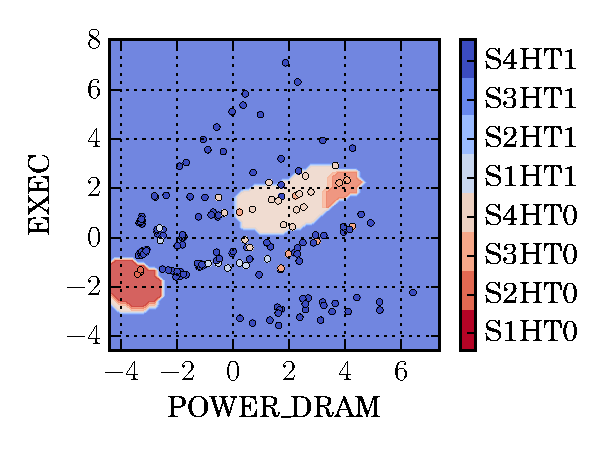
\includegraphics[width=0.3\columnwidth]{figs/classifiers/training_space_svm_ts.pdf}
  \label{fig:feat-svm-ts}
  % \vspace{ -1.5em }
  }
  % \\
  % \vskip -1.5em
  \hspace*{0.1cm}
  \subfloat[DVFS only, recall=0.645.]
  {\centering 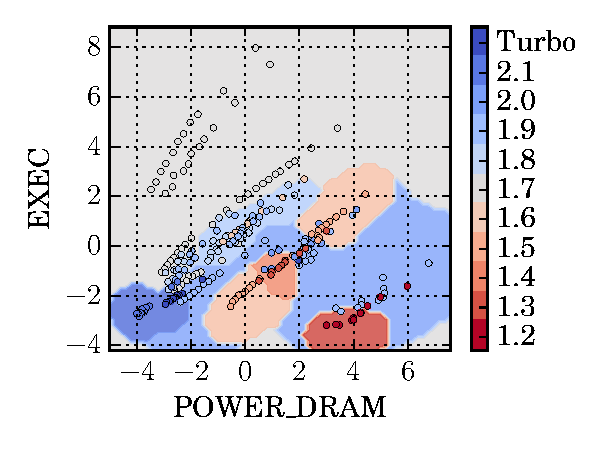
\includegraphics[width=0.3\columnwidth]{figs/classifiers/training_space_svm_dvfs.pdf}
  \label{fig:feat-space-svm-dvfs}
  % \vspace{ -1.5em }
}
\caption{Training data and learned decision boundaries for SVM when classifying for taskset and DVFS separately.}
\label{fig:feat-space-svm-separate}
% \vskip -1.0em
\end{figure}

An alternative approach is for one classifier to predict the taskset, and a separate classifier to predict the DVFS frequency.
\figref{feat-space-svm-separate} visualizes the training and recall for SVM (like \figref{feat-space-svm} in \secref{challenges-learning}) using separate classifiers.
Note that there are fewer data points, as DVFS is fixed at TurboBoost when training for taskset, and taskset is fixed at all sockets and HyperThreads when training for DVFS.
Taskset's recall is quite good, while DVFS is not as good as before.
There is, of course, additional overhead in running two classifiers instead of one, but \secref{classifiers-eval-overhead} demonstrated that data processing overhead is not significant, and there is still only a single instance of PCM and the actuators running.

\begin{figure}[t]
  \centering
  \begin{tikzpicture}
\definecolor{s1}{RGB}{228, 26, 28}
\definecolor{s2}{RGB}{55, 126, 184}
\definecolor{s3}{RGB}{77, 175, 74}
\definecolor{s4}{RGB}{152, 78, 163}
\definecolor{s5}{RGB}{255, 127, 0}

\begin{groupplot}[
    group style={
        group name=plots,
        group size=1 by 1,
        xlabels at=edge bottom,
        xticklabels at=edge bottom,
        vertical sep=5pt
    },
% axis x line* = bottom,
xlabel near ticks,
major x tick style = transparent,
xlabel={},
height=3.5cm,
width=0.95\columnwidth,
xmin=0.5,
xmax=5.5,
enlargelimits=false,
tick align = outside,
tick style={white},
ylabel style={align=center},
ytick=\empty,
ymin=0.6,
ymax=1.1,
ytick={0.6,0.7,0.8,0.9,1.0,1.1},
yticklabels={0.6,0.7,0.8,0.9,1.0,1.1},
legend cell align=left, 
legend style={ column sep=1ex },
ymajorgrids,
grid style={dashed},
]

\nextgroupplot[ylabel={Energy \\ (Normalized)},
ybar=\pgflinewidth,
legend entries = {{Single},{Separate}},
legend style={draw=none,legend columns=5,at={(.5,1.4)},anchor=north},
bar width=8pt,
ylabel shift={0mm},
xticklabel shift={0pt},
x tick label style={rotate=35, anchor=east, font=\scriptsize},
xtick={1,2,3,4,5,6,7},
xticklabels={
{ET},
{GB},
{KNN},
{MLP},
{SVM},
},
execute at end plot={
% "Race":
\draw[thin, dashed] (axis cs:\pgfkeysvalueof{/pgfplots/xmin},1) -- (axis cs:\pgfkeysvalueof{/pgfplots/xmax},1);
% "Best static DVFS":
\draw[thick, dotted] (axis cs:\pgfkeysvalueof{/pgfplots/xmin},0.765646972) -- (axis cs:\pgfkeysvalueof{/pgfplots/xmax},0.765646972);
% "ET_SVM"
\draw[thin, solid] (axis cs:\pgfkeysvalueof{/pgfplots/xmin},0.8288250669) -- (axis cs:\pgfkeysvalueof{/pgfplots/xmax},0.8288250669);
% hack to reset column line style (ghostscript seems to use last formatting as line style, e.g. dashed or dotted instead of solid)
\draw[thin, solid] (axis cs:\pgfkeysvalueof{/pgfplots/xmin},\pgfkeysvalueof{/pgfplots/ymin}) -- (axis cs:\pgfkeysvalueof{/pgfplots/xmax},\pgfkeysvalueof{/pgfplots/ymin});
},
]
\addplot table[x index=0,y index=7, col sep=tab] {img/classifiers/compare_interval/compare_5s.txt};
\addplot table[x index=0,y index=7, col sep=tab] {img/classifiers/compare_pca/sep_clfs.txt};

\end{groupplot}

\end{tikzpicture}
  \caption{Average energy consumption when using a single or separate classifiers for system knobs (lower is better).}
  \label{fig:separate-clfs}
  % \vskip -1.0em
\end{figure}

\figref{separate-clfs} quantifies the behavior when we use two separate classifiers simultaneously.
In each case, the same type of classifier is used for both taskset and DVFS prediction.
In three of five cases, $Separate$ actually outperforms the $Single$ approach.
However, it is also possible for $Separate$ to perform rather poorly, as seen with the MLP classifier.
The average MLP behavior is representative of the applications tested, \ie not caused by an outlier---in three of the four applications evaluated, MLP classifying taskset and DVFS separately performed worse than the \emph{race-to-idle} heuristic.
Of course, taskset and DVFS prediction may benefit from using different classification algorithms.
We tested taskset-only and DVFS-only classifiers in isolation and empirically determined that, for our system and applications, the ET classifier works best for taskset prediction and the SVM classifier works best for DVFS prediction.
The solid horizontal line indicates the energy consumption for this ET/SVM classifier mix.
While this avoided the poor results seen with MLP, it actually performed slightly worse than three of the four remaining $Single$ classifier approaches.
Using a single, unified classifier that learns both taskset and DVFS together ultimately produces more reliable predictions.


\subsection{Discussion of Results and Limitations}
\label{sec:eval-discuss}

Our evaluation demonstrates that machine learning classification driven by low-level features is an effective approach for improving energy efficiency.
In fact, a variety of different classifiers are useful for predicting energy-efficient system settings at runtime, even without classifier tuning.
No single classifier appears to have a clear advantage over others, though future work on fine-tuning the training data and classifiers, combined with evaluations on other platforms, may eventually produce a near-optimal implementation.

We also did not attempt to optimize the runtime's overhead---reading performance counters, data transformations, or system actuation.
Although low, there is still room for improvement, which could support faster sampling and prediction intervals and further improve energy consumption.

We currently only manage socket/core allocation at system-level.
Because applications are launched with a fixed number of threads, those threads are forced to share compute cores when we bind applications to fewer sockets or disable HyperThreads during runtime.
This over-subscription is usually not as efficient as matching the thread count to the available cores, \eg running 80 threads on our 80 physical cores is more efficient that binding 160 threads to those 80 cores.
Integration with application-level parallelism can further improve energy efficiency and reduce resource contention when binding applications to smaller tasksets \cite{Sridharan2013}.
% \TODO{Anything on memory allocation/interleaving? We really don't have a solution to this problem when using dynamic taskset.}

On large systems such as our evaluation platform, the processor and DRAM consume the majority of system power, which we are able to measure \cite{RAPL,PCMGit}.
There are other components like hard disks and network interfaces that are not currently accounted for.
While it is not common practice to instrument these other components for power/energy monitoring, such feedback could help resource management solutions achieve better total energy efficiency.

